\documentclass[11pt,a4paper]{article}
\usepackage[T1]{fontenc}
\usepackage[latin1]{inputenc}
\usepackage{lmodern}
\usepackage{a4wide}
\usepackage{float}
\usepackage[dvips]{graphicx}

\usepackage[
pdfauthor={ACE Project Team},
pdftitle={Project Manual},
pdfcreator={pdftex},
]{hyperref}

\usepackage{sectsty}
\allsectionsfont{\sffamily}

\usepackage{fancyheadings} 
\pagestyle{fancy} 
\lhead{\textsf{\textbf{ACE} \\ \small{a collaborative editor}}}
\chead{}
\rhead{
\parbox[c]{3cm}{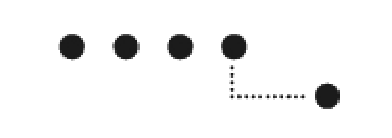
\includegraphics[height=0.875cm,width=3cm]{../../images/logo_BFH.eps}}
\parbox[c]{2.2cm}
{\tiny{\textsf{Berner Fachhochschule \\
Hochschule f�r \\
Technik und Informatik}}}}
\lfoot{}
\cfoot{\textsf{\thepage}}
\rfoot{}
\setlength{\headrulewidth}{0.6pt}
\setlength{\footrulewidth}{0.6pt}
\setlength{\topmargin}{-50pt}
\addtolength{\headheight}{50pt}

\usepackage{colortbl}

\newcommand{\headercol}[2]{\multicolumn{1}{|>{\bfseries\columncolor[gray]{0.82}}p{#1}|}{\textsf{#2}}}
\newcommand{\ace}[0]{\emph{ACE }}



\begin{document}

\setlength{\parindent}{0pt}

\begin{titlepage}
\thispagestyle{empty}
  
\includegraphics[height=1.5in]{../images/pix.eps}

  \begin{center}

    {\fontsize{40}{45} \textbf{\textsf{ACE}}} \\
    \textsf{a collaborative editor} \\
        
    \vspace{36pt}
        
    {\huge{\textbf{\textsf{}}}} \\

    \vspace{36pt}

	\textsf{Berne University of Applied Sciences} \\
    \textsf{School of Engineering and Information Technology} \\
    
  \end{center}

  \vfill
  
  \begin{tabular}{ll}
   \hline

   \\

   \multicolumn{1}{>{\bfseries}p{1.5in}}{\textsf{Date:}} &
   \multicolumn{1}{>{}p{4.3in}}{\textsf{08.11.2005}}          \\
   
   \\
   
   \multicolumn{1}{>{\bfseries}p{1.5in}}{\textsf{Version:}}     &   
   \multicolumn{1}{>{}p{4.3in}}{\textsf{0.1}}                 \\

   \\
   
   \multicolumn{1}{>{\bfseries}p{1.5in}}{\textsf{Projectteam:}}                 &
   \multicolumn{1}{>{}p{4.3in}}{\textsf{Mark Bigler (biglm2@hta-bi.bfh.ch)}}  \\
   \multicolumn{1}{>{\bfseries}p{1.5in}}{}                                      &
   \multicolumn{1}{>{}p{4.3in}}{\textsf{Simon Raess (rasss@hta-bi.bfh.ch)}}    \\
   \multicolumn{1}{>{\bfseries}p{1.5in}}{}                                      &
   \multicolumn{1}{>{}p{4.3in}}{\textsf{Lukas Zbinden (zbinl@hta-bi.bfh.ch)}} \\   
   
   \\
   
   \multicolumn{1}{>{\bfseries}p{1.5in}}{\textsf{Receivers:}}                       &
   \multicolumn{1}{>{}p{4.3in}}{\textsf{Jean-Paul Dubois (doj@hta-bi.bfh.ch)}}       \\
   \multicolumn{1}{>{\bfseries}p{1.5in}}{}                                          &
   \multicolumn{1}{>{}p{4.3in}}{\textsf{Claude Fuhrer (frc@hta-bi.bfh.ch)}}       \\

   \\
   
   \multicolumn{1}{>{\bfseries}p{1.5in}}{\textsf{Location:}}               &   
   \multicolumn{1}{>{}p{4.3in}}{\textsf{Subversion Repository}} \\

   \\  
   
   \hline
  \end{tabular}

\end{titlepage}


\tableofcontents

\newpage

\section{Introduction}

\section{Project Documentation}
The following list contains all the relevant documents for the diploma project ACE.
\begin{itemize}
 \item System Requirements
 \item Project Manual (this document)
 \item User Manual
 \item Final Report
\end{itemize}

\subsection{System Requirements}
\begin{itemize}
 \item definition of project goals
 \item description of functionality
\end{itemize}

\subsection{Project Manual}
\begin{itemize}
 \item list of delivered documents
 \item project plan: work phases, project organization
 \item used methods and tools
 \item standards, guidelines, and conventions
\end{itemize}

\subsection{User Manual}
\begin{itemize}
 \item instructions how to use the application (end users)
 \item instructions how to build and run the application (developers)
\end{itemize}

\subsection{Final Report}
The final report contains all the technical documentation of the project.
\begin{itemize}
 \item abstract
 \item description of goals and content of project
 \item description of implemented solution (implementation decisions)
 \item application architecture and design
 \item test concept and results
 \item references
 \item glossary
\end{itemize}


\section{Persons}

\begin{table}[H]
 \begin{center}
 \begin{tabular}{|l|l|l|l|}
 \hline
 Contractor             &  J.-P. Dubois     & \href{mailto:doj@bfh.ch}{doj@bfh.ch} \\
                        &                   &  +41 32 321 62 82 \\
 \hline
 Project Lead           &  S. Raess         & \href{mailto:rasss@bfh.ch}{rasss@bfh.ch} \\
 \hline
 Project Team           &  M. Bigler        & \href{mailto:biglm2@bfh.ch}{biglm2@bfh.ch} \\ 
                        &  S. Raess         & \href{mailto:rasss@bfh.ch}{rasss@bfh.ch} \\
                        &  L. Zbinden       & \href{mailto:zbinl@bfh.ch}{zbinl@bfh.ch} \\
 \hline
 Project Coach          &  J.-P. Dubois     & \href{mailto:doj@bfh.ch}{doj@bfh.ch} \\
                        &  C. Fuhrer        & \href{frc@bfh.ch}{frc@bfh.ch} \\
 \hline
 \end{tabular}
 \end{center}
 \caption{Project Organization}
 \label{table: Project Organization}
\end{table}


\section{Project Organization}

In the diploma project we use a lifecycle model tailored to our needs. It is an iterative
model with a very short iteration time (2 weeks). Three iterations are planned where the last
iteration consists mainly of bugfixes and/or usability improvements. Each phase is
completed by a milestone (see the milestone plan \ref{sect:Milestone Plan}). At the end of
the third phase, the application will be finished according to the defined goals (see
\emph{System Requirements} document).

At the beginning we invest some time to initialize the project and to create a concept
for the implementation. The concept includes the design of the interfaces between the
three layers into which ACE is split: application, collaboration, and network layer.

In the first iteration, we start implementing the different layers. Each layer is
implemented by a different team member for which he is responsible. If one team member
finishes a layer earlier, he helps another team member. The following table shows
who is responsible for which layer. The layer lead developer is responsible that his
layer is completed in time and fully functioning. However this does not mean that
a layer is implemented 100 percent by one person.

\begin{table}[H]
 \centering
 \begin{tabular}{|l|l|l|l|}
  \hline
  \headercol{2in}{Layer}        & 
  \headercol{2in}{Lead Developer}  \\ 
  \hline
   Application Layer         & Mark Bigler   \\
  \hline
   Collaboration Layer       & Simon Raess   \\
  \hline
   Network Layer             & Lukas Zbinden \\
  \hline
 \end{tabular}
 \caption{Layers and Lead Developers}
 \label{Layers and Lead Developers}
\end{table}

\subsection{Layers}

ACE is split into three independent layers. Each layer has a well-defined interface
between the adjoining layers and well-defined responsibilities. 
It should be possible to replace a layer implementation without affecting the other 
layers.

\begin{figure}[H]
 \centering
 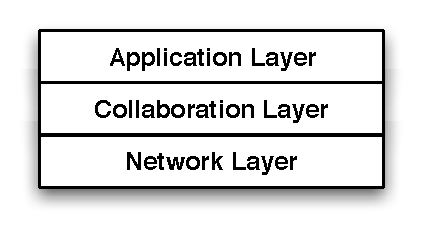
\includegraphics[width=6.6cm,height=3.42cm]{../images/layers.eps}
 \caption{The Layers of ACE}
\end{figure}

\paragraph{Application Layer:} The application layer consists mainly in the graphical
user interface. ACE itself will have a layer implementation based on a Java Swing GUI.

\paragraph{Collaboration Layer:} The collaboration layer provides the collaborative
editing functionality to the application layer. It hosts the core consistency
control algorithm, which is based on the concept of operational transformation.
By replacing the collaboration layer it would be theoretically possible to replace
the employed consistency control algorithm. Further it uses the network layer
for all network related functionality.

\paragraph{Network Layer:} The network layer is the lowest layer of ACE. It provides
networking functionality to the collaboration layer. The two most important features
are discovery of users and documents as well as communication with other users and
sessions. Replacing the network layer allows to use a different network technology 
and/or a different protocol.


\section{Project Plan}

\begin{figure}[H]
 \centering
 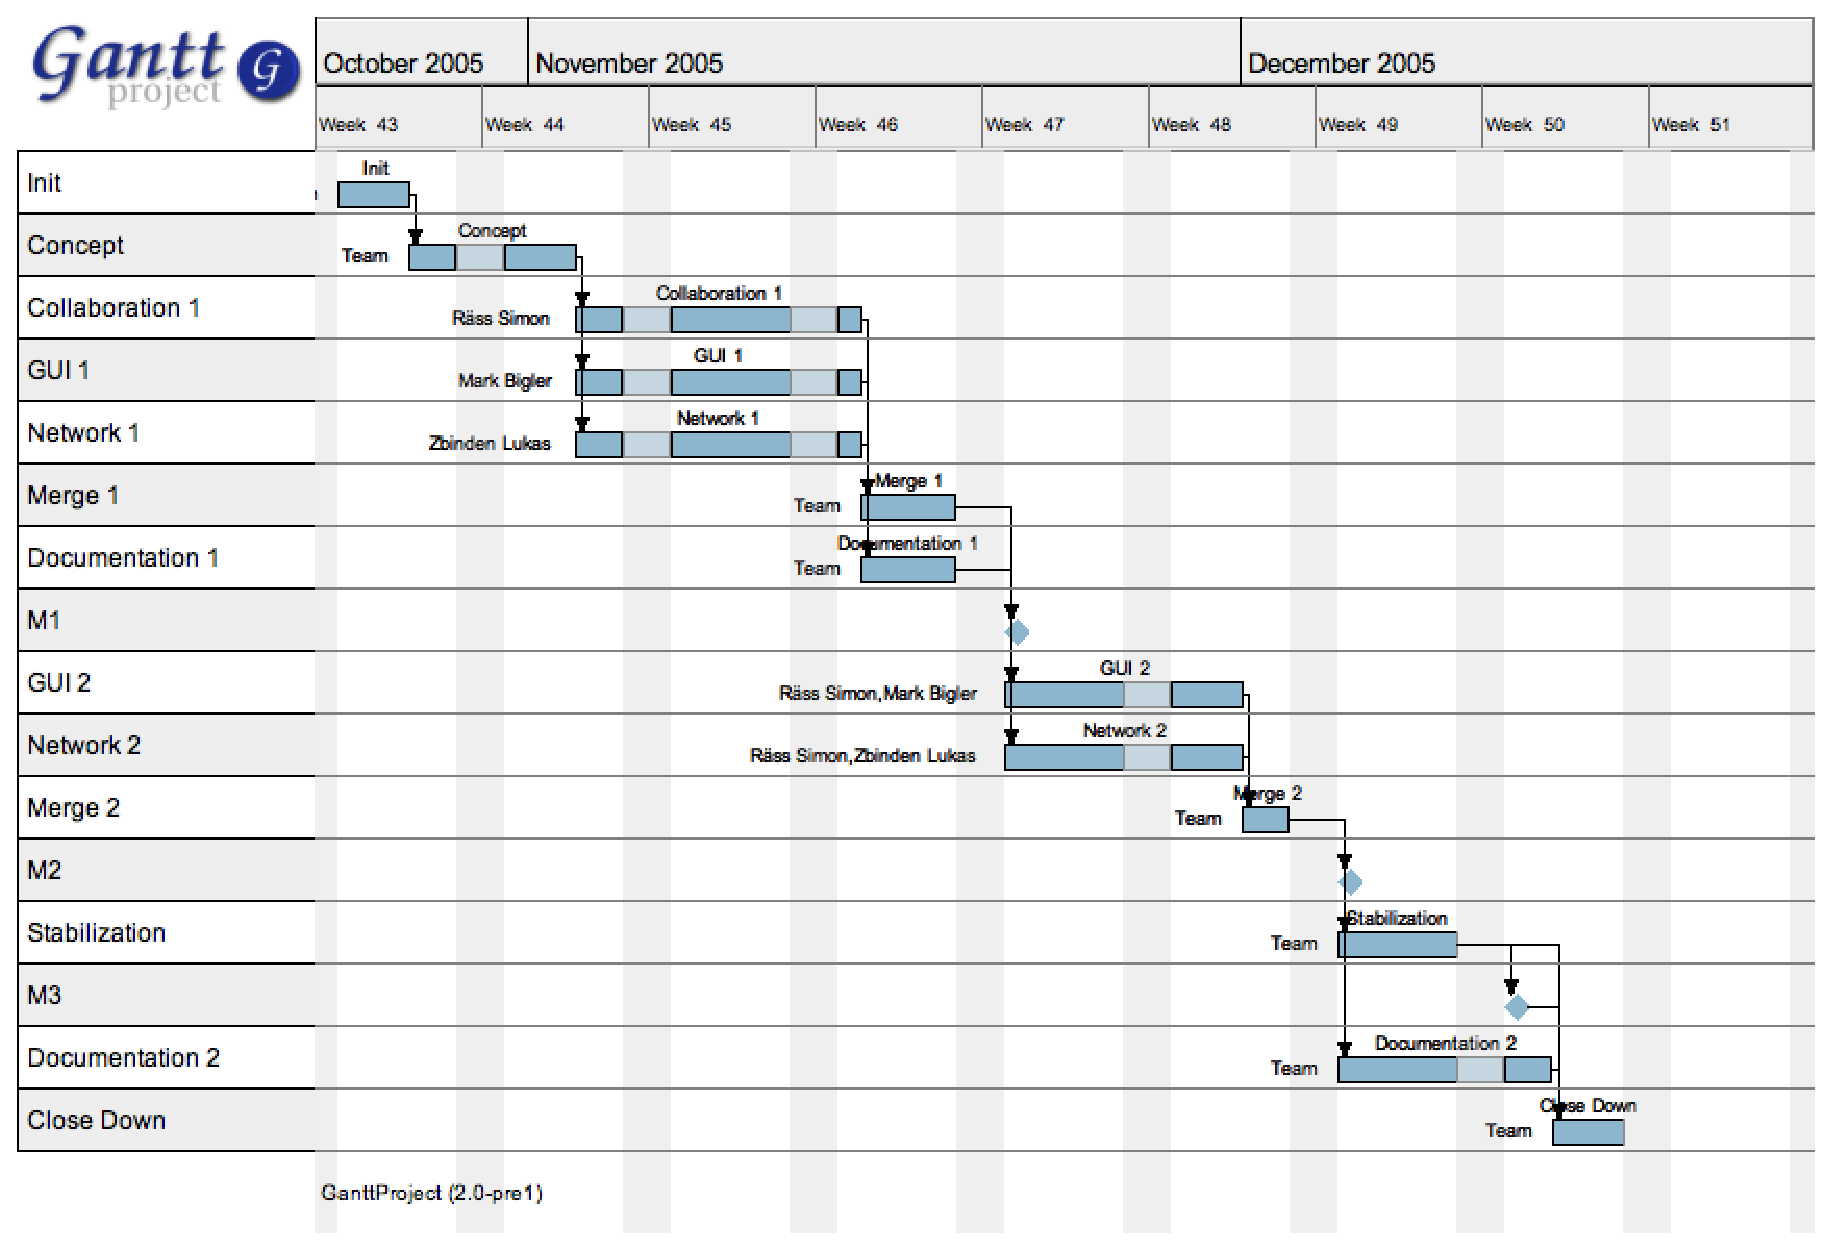
\includegraphics[height=379pt,width=585pt,angle=90]{../images/projectmanagement/gantt.eps}
 \caption{Project Plan}
\end{figure}
\newpage

\subsection{Milestone Plan}
\label{sect:Milestone Plan}

In the diploma project there are three milestones. Each milestone is at the end of an iteration.

\subsubsection{Milestone M1}

The scheduled release date of Milestone 1 is: 21.11.2005. Milestone 1 includes the text editor with
all the discovery related functionality. Although it will be possible to publish local documents
it is not yet possible to join the shared documents.

\begin{itemize}
 \item create new documents
 \item load and save documents
 \item open multiple documents at the same time
 \item cut/copy/paste
 \item about information
 \item publish local documents
 \item automatic discovery of other running instances of ACE on a local area network (user discovery)
 \item automatic discovery of published documents of other running instances of ACE (document discovery)
\end{itemize}

\subsubsection{Milestone M2}

The scheduled release date of Milestone 2 is: 05.12.2005. Milestone 2 adds the collaboration functionality
to the text editor, including joining documents, collaborative editing, and awareness information.

\begin{itemize}
 \item join published documents
 \item collaborative editing in a shared document
 \item awareness information
 \item leave joined documents
 \item kick users
\end{itemize}

\subsubsection{Milestone M3}

The scheduled release date of Milestone 3 is: 12.12.2005. Milestone 3 incorporates mainly bugfixes and
usability improvements based on feedback from testing.

\begin{itemize}
 \item bug fixes
 \item usability improvements
 \item design
 \item optional goals
\end{itemize}

\subsection{Work Packages}

\subsubsection{Workpackage: Initialization}
\begin{table}[H]
 \begin{tabular}{|l|l|l|l|}
  \hline
    \multicolumn{3}{|>{\columncolor[gray]{0.82}}p{5.85in}|}{\bfseries{\textsf{Work Package: Initialization}}} \\
  \hline
    \multicolumn{1}{|p{1in}|}{\bfseries{\textsf{Assigned To}}} &
    \multicolumn{2}{|p{4.5in}|}{Project Team} \\
  \hline
    \multicolumn{1}{|p{1in}|}{\bfseries{\textsf{Input}}} &
    \multicolumn{2}{|p{4.5in}|}{} \\
  \hline
    \multicolumn{1}{|p{1in}|}{\bfseries{\textsf{Output}}} &
    \multicolumn{2}{|p{4.5in}|}{Development Environment} \\
    \multicolumn{1}{|p{1in}|}{} &
    \multicolumn{2}{|p{4.5in}|}{Project Server} \\
    \multicolumn{1}{|p{1in}|}{} &
    \multicolumn{2}{|p{4.5in}|}{Updated Project Website} \\
    
  \hline \hline
    \multicolumn{1}{|>{\columncolor[gray]{0.82}}p{1in}|}{} &
    \multicolumn{1}{|>{\columncolor[gray]{0.82}}p{3.5in}|}{\bfseries{\textsf{Description}}} &
    \multicolumn{1}{|>{\columncolor[gray]{0.82}}p{1in}|}{\bfseries{\textsf{Time}}} \\
  \hline
    \multicolumn{1}{|p{1in}|}{\bfseries{\textsf{Activities}}} &
    \multicolumn{1}{|p{3.5in}|}{Installing Cruise Control} &
    \multicolumn{1}{|p{1in}|}{0.5 Tage} \\
    \multicolumn{1}{|p{1in}|}{} &
    \multicolumn{1}{|p{3.5in}|}{Installing Issue Tracker and Wiki} &
    \multicolumn{1}{|p{1in}|}{1 Tag} \\
    \multicolumn{1}{|p{1in}|}{} &
    \multicolumn{1}{|p{3.5in}|}{Updating Project Website} &
    \multicolumn{1}{|p{1in}|}{1 Tag} \\
  \hline
    \multicolumn{1}{|p{1in}|}{\bfseries{\textsf{QA}}} &
    \multicolumn{1}{|p{3.5in}|}{} &
    \multicolumn{1}{|p{1in}|}{} \\
  \hline \hline
    \multicolumn{1}{|p{1in}|}{\bfseries{\textsf{Total}}} &
    \multicolumn{1}{|p{3.5in}|}{} &
    \multicolumn{1}{|p{1in}|}{4 Tage} \\
  \hline
 \end{tabular}
 \caption{Workpackage Initialization}
 \label{Workpackage Initialization}
\end{table}

%%
% total time for workpackage must be: 3 * 5 = 15 days
%
\subsubsection{Workpackage: Concept}
\begin{table}[H]
 \begin{tabular}{|l|l|l|l|}
  \hline
    \multicolumn{3}{|>{\columncolor[gray]{0.82}}p{5.85in}|}{\bfseries{\textsf{Work Package: Concept}}} \\
  \hline
    \multicolumn{1}{|p{1in}|}{\bfseries{\textsf{Assigned To}}} &
    \multicolumn{2}{|p{4.5in}|}{Project Team} \\
  \hline
    \multicolumn{1}{|p{1in}|}{\bfseries{\textsf{Input}}} &
    \multicolumn{2}{|p{4.5in}|}{} \\
  \hline
    \multicolumn{1}{|p{1in}|}{\bfseries{\textsf{Output}}} &
    \multicolumn{2}{|p{4.5in}|}{Design of Layer Interfaces} \\
    \multicolumn{1}{|p{1in}|}{} &
    \multicolumn{2}{|p{4.5in}|}{Prototypes} \\ 
    \multicolumn{1}{|p{1in}|}{} &
    \multicolumn{2}{|p{4.5in}|}{Project Manual} \\ 
    \multicolumn{1}{|p{1in}|}{} &
    \multicolumn{2}{|p{4.5in}|}{System Requirements} \\ 
  \hline \hline
    \multicolumn{1}{|>{\columncolor[gray]{0.82}}p{1in}|}{} &
    \multicolumn{1}{|>{\columncolor[gray]{0.82}}p{3.5in}|}{\bfseries{\textsf{Description}}} &
    \multicolumn{1}{|>{\columncolor[gray]{0.82}}p{1in}|}{\bfseries{\textsf{Time}}} \\
  \hline
    \multicolumn{1}{|p{1in}|}{\bfseries{\textsf{Activities}}} &
    \multicolumn{1}{|p{3.5in}|}{Writing Project Manual and System Requirements} &
    \multicolumn{1}{|p{1in}|}{1 Day} \\
    \multicolumn{1}{|p{1in}|}{} &
    \multicolumn{1}{|p{3.5in}|}{Designing Layer Interfaces} &
    \multicolumn{1}{|p{1in}|}{4 Days} \\
    \multicolumn{1}{|p{1in}|}{} &
    \multicolumn{1}{|p{3.5in}|}{Designing Layer Implementations} &
    \multicolumn{1}{|p{1in}|}{3 Days} \\
    \multicolumn{1}{|p{1in}|}{} &
    \multicolumn{1}{|p{3.5in}|}{Implementing Prototypes Network} &
    \multicolumn{1}{|p{1in}|}{2 Days} \\
    \multicolumn{1}{|p{1in}|}{} &
    \multicolumn{1}{|p{3.5in}|}{Implementing Prototypes GUI} &
    \multicolumn{1}{|p{1in}|}{2 Days} \\
  \hline
    \multicolumn{1}{|p{1in}|}{\bfseries{\textsf{QA}}} &
    \multicolumn{1}{|p{3.5in}|}{Design Review} &
    \multicolumn{1}{|p{1in}|}{3 Days} \\
  \hline \hline
    \multicolumn{1}{|p{1in}|}{\bfseries{\textsf{Total}}} &
    \multicolumn{1}{|p{3.5in}|}{} &
    \multicolumn{1}{|p{1in}|}{15 Days} \\
  \hline
 \end{tabular}
 \caption{Workpackage Concept}
 \label{Workpackage Concept}
\end{table}

%\include{wp/logic-1}
%%
% total time for workpackage must be: 8 days
%
\subsubsection{Workpackage: GUI 1}
\begin{table}[H]
 \begin{tabular}{|l|l|l|l|}
  \hline
    \multicolumn{3}{|>{\columncolor[gray]{0.82}}p{5.85in}|}{\bfseries{\textsf{Work Package: GUI 1}}} \\
  \hline
    \multicolumn{1}{|p{1in}|}{\bfseries{\textsf{Assigned To}}} &
    \multicolumn{2}{|p{4.5in}|}{Mark Bigler} \\
  \hline
    \multicolumn{1}{|p{1in}|}{\bfseries{\textsf{Input}}} &
    \multicolumn{2}{|p{4.5in}|}{Design of Layer Interfaces} \\
  \hline
    \multicolumn{1}{|p{1in}|}{\bfseries{\textsf{Output}}} &
    \multicolumn{2}{|p{4.5in}|}{Implementation Version M1} \\    
  \hline \hline
    \multicolumn{1}{|>{\columncolor[gray]{0.82}}p{1in}|}{} &
    \multicolumn{1}{|>{\columncolor[gray]{0.82}}p{3.5in}|}{\bfseries{\textsf{Description}}} &
    \multicolumn{1}{|>{\columncolor[gray]{0.82}}p{1in}|}{\bfseries{\textsf{Time}}} \\
  \hline
    \multicolumn{1}{|p{1in}|}{\bfseries{\textsf{Activities}}} &
    \multicolumn{1}{|p{3.5in}|}{} &
    \multicolumn{1}{|p{1in}|}{} \\
    \multicolumn{1}{|p{1in}|}{} &
    \multicolumn{1}{|p{3.5in}|}{} &
    \multicolumn{1}{|p{1in}|}{} \\
    \multicolumn{1}{|p{1in}|}{} &
    \multicolumn{1}{|p{3.5in}|}{} &
    \multicolumn{1}{|p{1in}|}{} \\
  \hline
    \multicolumn{1}{|p{1in}|}{\bfseries{\textsf{QA}}} &
    \multicolumn{1}{|p{3.5in}|}{} &
    \multicolumn{1}{|p{1in}|}{} \\
  \hline \hline
    \multicolumn{1}{|p{1in}|}{\bfseries{\textsf{Total}}} &
    \multicolumn{1}{|p{3.5in}|}{} &
    \multicolumn{1}{|p{1in}|}{8 Days} \\
  \hline
 \end{tabular}
 \caption{Workpackage GUI 1}
 \label{Workpackage GUI 1}
\end{table}

%%
% total time for workpackage must be: 8 days
%
\subsubsection{Workpackage: Network 1}
\begin{table}[H]
 \begin{tabular}{|l|l|l|l|}
  \hline
    \multicolumn{3}{|>{\columncolor[gray]{0.82}}p{5.85in}|}{\bfseries{\textsf{Work Package: Network 1}}} \\
  \hline
    \multicolumn{1}{|p{1in}|}{\bfseries{\textsf{Assigned To}}} &
    \multicolumn{2}{|p{4.5in}|}{Lukas Zbinden} \\
  \hline
    \multicolumn{1}{|p{1in}|}{\bfseries{\textsf{Input}}} &
    \multicolumn{2}{|p{4.5in}|}{Design of Layer Interfaces} \\
  \hline
    \multicolumn{1}{|p{1in}|}{\bfseries{\textsf{Output}}} &
    \multicolumn{2}{|p{4.5in}|}{Implementation Version M1} \\    
  \hline \hline
    \multicolumn{1}{|>{\columncolor[gray]{0.82}}p{1in}|}{} &
    \multicolumn{1}{|>{\columncolor[gray]{0.82}}p{3.5in}|}{\bfseries{\textsf{Description}}} &
    \multicolumn{1}{|>{\columncolor[gray]{0.82}}p{1in}|}{\bfseries{\textsf{Time}}} \\
  \hline
    \multicolumn{1}{|p{1in}|}{\bfseries{\textsf{Activities}}} &
    \multicolumn{1}{|p{3.5in}|}{} &
    \multicolumn{1}{|p{1in}|}{} \\
    \multicolumn{1}{|p{1in}|}{} &
    \multicolumn{1}{|p{3.5in}|}{} &
    \multicolumn{1}{|p{1in}|}{} \\
    \multicolumn{1}{|p{1in}|}{} &
    \multicolumn{1}{|p{3.5in}|}{} &
    \multicolumn{1}{|p{1in}|}{} \\
  \hline
    \multicolumn{1}{|p{1in}|}{\bfseries{\textsf{QA}}} &
    \multicolumn{1}{|p{3.5in}|}{} &
    \multicolumn{1}{|p{1in}|}{} \\
  \hline \hline
    \multicolumn{1}{|p{1in}|}{\bfseries{\textsf{Total}}} &
    \multicolumn{1}{|p{3.5in}|}{} &
    \multicolumn{1}{|p{1in}|}{8 Days} \\
  \hline
 \end{tabular}
 \caption{Workpackage Network 1}
 \label{Workpackage Network 1}
\end{table}

%%
% total time for workpackage must be: 3 * 2 = 6 days
%
\subsubsection{Workpackage: Merge 1}
\begin{table}[H]
 \begin{tabular}{|l|l|l|l|}
  \hline
    \multicolumn{3}{|>{\columncolor[gray]{0.82}}p{5.85in}|}{\bfseries{\textsf{Work Package: Merge 1}}} \\
  \hline
    \multicolumn{1}{|p{1in}|}{\bfseries{\textsf{Assigned To}}} &
    \multicolumn{2}{|p{4.5in}|}{Project Team} \\
  \hline
    \multicolumn{1}{|p{1in}|}{\bfseries{\textsf{Input}}} &
    \multicolumn{2}{|p{4.5in}|}{Implementation Collaboration Layer} \\
    \multicolumn{1}{|p{1in}|}{} &
    \multicolumn{2}{|p{4.5in}|}{GUI 1} \\
    \multicolumn{1}{|p{1in}|}{} &
    \multicolumn{2}{|p{4.5in}|}{Network 1} \\
  \hline
    \multicolumn{1}{|p{1in}|}{\bfseries{\textsf{Output}}} &
    \multicolumn{2}{|p{4.5in}|}{Product Release Milestone 1} \\    
  \hline \hline
    \multicolumn{1}{|>{\columncolor[gray]{0.82}}p{1in}|}{} &
    \multicolumn{1}{|>{\columncolor[gray]{0.82}}p{3.5in}|}{\bfseries{\textsf{Description}}} &
    \multicolumn{1}{|>{\columncolor[gray]{0.82}}p{1in}|}{\bfseries{\textsf{Time}}} \\
  \hline
    \multicolumn{1}{|p{1in}|}{\bfseries{\textsf{Activities}}} &
    \multicolumn{1}{|p{3.5in}|}{Merging Changes} &
    \multicolumn{1}{|p{1in}|}{1 Day} \\
    \multicolumn{1}{|p{1in}|}{} &
    \multicolumn{1}{|p{3.5in}|}{Fixing Integration Problems} &
    \multicolumn{1}{|p{1in}|}{2.5 Days} \\
    \multicolumn{1}{|p{1in}|}{} &
    \multicolumn{1}{|p{3.5in}|}{Updating Project Website} &
    \multicolumn{1}{|p{1in}|}{0.5 Days} \\
  \hline
    \multicolumn{1}{|p{1in}|}{\bfseries{\textsf{QA}}} &
    \multicolumn{1}{|p{3.5in}|}{Integration Testing} &
    \multicolumn{1}{|p{1in}|}{2 Days} \\
  \hline \hline
    \multicolumn{1}{|p{1in}|}{\bfseries{\textsf{Total}}} &
    \multicolumn{1}{|p{3.5in}|}{} &
    \multicolumn{1}{|p{1in}|}{6 Days} \\
  \hline
 \end{tabular}
 \caption{Workpackage Merge 1}
 \label{Workpackage Merge 1}
\end{table}

%%
% total time for workpackage must be: 12 days
%
\subsubsection{Workpackage: GUI 2}
\begin{table}[H]
 \begin{tabular}{|l|l|l|l|}
  \hline
    \multicolumn{3}{|>{\columncolor[gray]{0.82}}p{5.85in}|}{\bfseries{\textsf{Work Package: GUI 2}}} \\
  \hline
    \multicolumn{1}{|p{1in}|}{\bfseries{\textsf{Assigned To}}} &
    \multicolumn{2}{|p{4.5in}|}{Mark Bigler} \\
    \multicolumn{1}{|p{1in}|}{} &
    \multicolumn{2}{|p{4.5in}|}{Simon Raess (50\%)} \\
  \hline
    \multicolumn{1}{|p{1in}|}{\bfseries{\textsf{Input}}} &
    \multicolumn{2}{|p{4.5in}|}{} \\
  \hline
    \multicolumn{1}{|p{1in}|}{\bfseries{\textsf{Output}}} &
    \multicolumn{2}{|p{4.5in}|}{} \\
    \multicolumn{1}{|p{1in}|}{} &
    \multicolumn{2}{|p{4.5in}|}{} \\
    \multicolumn{1}{|p{1in}|}{} &
    \multicolumn{2}{|p{4.5in}|}{} \\
  \hline \hline
    \multicolumn{1}{|>{\columncolor[gray]{0.82}}p{1in}|}{} &
    \multicolumn{1}{|>{\columncolor[gray]{0.82}}p{3.5in}|}{\bfseries{\textsf{Description}}} &
    \multicolumn{1}{|>{\columncolor[gray]{0.82}}p{1in}|}{\bfseries{\textsf{Time}}} \\
  \hline
    \multicolumn{1}{|p{1in}|}{\bfseries{\textsf{Activities}}} &
    \multicolumn{1}{|p{3.5in}|}{} &
    \multicolumn{1}{|p{1in}|}{} \\
    \multicolumn{1}{|p{1in}|}{} &
    \multicolumn{1}{|p{3.5in}|}{} &
    \multicolumn{1}{|p{1in}|}{} \\
    \multicolumn{1}{|p{1in}|}{} &
    \multicolumn{1}{|p{3.5in}|}{} &
    \multicolumn{1}{|p{1in}|}{} \\
  \hline
    \multicolumn{1}{|p{1in}|}{\bfseries{\textsf{QA}}} &
    \multicolumn{1}{|p{3.5in}|}{} &
    \multicolumn{1}{|p{1in}|}{} \\
  \hline \hline
    \multicolumn{1}{|p{1in}|}{\bfseries{\textsf{Total}}} &
    \multicolumn{1}{|p{3.5in}|}{} &
    \multicolumn{1}{|p{1in}|}{12 Days} \\
  \hline
 \end{tabular}
 \caption{Workpackage GUI 2}
 \label{Workpackage GUI 2}
\end{table}

%%
% total time for workpackage must be: 8 + 4 = 12 days
%
\subsubsection{Workpackage: Network 2}
\begin{table}[H]
 \begin{tabular}{|l|l|l|l|}
  \hline
    \multicolumn{3}{|>{\columncolor[gray]{0.82}}p{5.85in}|}{\bfseries{\textsf{Work Package: Network 2}}} \\
  \hline
    \multicolumn{1}{|p{1in}|}{\bfseries{\textsf{Assigned To}}} &
    \multicolumn{2}{|p{4.5in}|}{Lukas Zbinden} \\
    \multicolumn{1}{|p{1in}|}{} &
    \multicolumn{2}{|p{4.5in}|}{Simon Raess (50\%)} \\
  \hline
    \multicolumn{1}{|p{1in}|}{\bfseries{\textsf{Input}}} &
    \multicolumn{2}{|p{4.5in}|}{} \\
  \hline
    \multicolumn{1}{|p{1in}|}{\bfseries{\textsf{Output}}} &
    \multicolumn{2}{|p{4.5in}|}{} \\
    \multicolumn{1}{|p{1in}|}{} &
    \multicolumn{2}{|p{4.5in}|}{} \\
    \multicolumn{1}{|p{1in}|}{} &
    \multicolumn{2}{|p{4.5in}|}{} \\
    
  \hline \hline
    \multicolumn{1}{|>{\columncolor[gray]{0.82}}p{1in}|}{} &
    \multicolumn{1}{|>{\columncolor[gray]{0.82}}p{3.5in}|}{\bfseries{\textsf{Description}}} &
    \multicolumn{1}{|>{\columncolor[gray]{0.82}}p{1in}|}{\bfseries{\textsf{Time}}} \\
  \hline
    \multicolumn{1}{|p{1in}|}{\bfseries{\textsf{Activities}}} &
    \multicolumn{1}{|p{3.5in}|}{} &
    \multicolumn{1}{|p{1in}|}{} \\
    \multicolumn{1}{|p{1in}|}{} &
    \multicolumn{1}{|p{3.5in}|}{} &
    \multicolumn{1}{|p{1in}|}{} \\
    \multicolumn{1}{|p{1in}|}{} &
    \multicolumn{1}{|p{3.5in}|}{} &
    \multicolumn{1}{|p{1in}|}{} \\
  \hline
    \multicolumn{1}{|p{1in}|}{\bfseries{\textsf{QA}}} &
    \multicolumn{1}{|p{3.5in}|}{} &
    \multicolumn{1}{|p{1in}|}{} \\
  \hline \hline
    \multicolumn{1}{|p{1in}|}{\bfseries{\textsf{Total}}} &
    \multicolumn{1}{|p{3.5in}|}{} &
    \multicolumn{1}{|p{1in}|}{12 Days} \\
  \hline
 \end{tabular}
 \caption{Workpackage Network 2}
 \label{Workpackage Network 2}
\end{table}

%%
% total time for workpackage must be: 3 * 2 = 6 days
%
\subsubsection{Workpackage: Merge 2}
\begin{table}[H]
 \begin{tabular}{|l|l|l|l|}
  \hline
    \multicolumn{3}{|>{\columncolor[gray]{0.82}}p{5.85in}|}{\bfseries{\textsf{Work Package: Merge 2}}} \\
  \hline
    \multicolumn{1}{|p{1in}|}{\bfseries{\textsf{Assigned To}}} &
    \multicolumn{2}{|p{4.5in}|}{Project Team} \\
  \hline
    \multicolumn{1}{|p{1in}|}{\bfseries{\textsf{Input}}} &
    \multicolumn{2}{|p{4.5in}|}{GUI 2} \\
    \multicolumn{1}{|p{1in}|}{} &
    \multicolumn{2}{|p{4.5in}|}{Network 2} \\
  \hline
    \multicolumn{1}{|p{1in}|}{\bfseries{\textsf{Output}}} &
    \multicolumn{2}{|p{4.5in}|}{Product Release Milestone 2} \\
  \hline \hline
    \multicolumn{1}{|>{\columncolor[gray]{0.82}}p{1in}|}{} &
    \multicolumn{1}{|>{\columncolor[gray]{0.82}}p{3.5in}|}{\bfseries{\textsf{Description}}} &
    \multicolumn{1}{|>{\columncolor[gray]{0.82}}p{1in}|}{\bfseries{\textsf{Time}}} \\
  \hline
    \multicolumn{1}{|p{1in}|}{\bfseries{\textsf{Activities}}} &
    \multicolumn{1}{|p{3.5in}|}{Merging Changes} &
    \multicolumn{1}{|p{1in}|}{1 Day} \\
    \multicolumn{1}{|p{1in}|}{} &
    \multicolumn{1}{|p{3.5in}|}{Fixing Integration Problems} &
    \multicolumn{1}{|p{1in}|}{2.5 Days} \\
    \multicolumn{1}{|p{1in}|}{} &
    \multicolumn{1}{|p{3.5in}|}{Updating Project Website} &
    \multicolumn{1}{|p{1in}|}{0.5 Days} \\
  \hline
    \multicolumn{1}{|p{1in}|}{\bfseries{\textsf{QA}}} &
    \multicolumn{1}{|p{3.5in}|}{Integration Testing} &
    \multicolumn{1}{|p{1in}|}{2 Days} \\
  \hline \hline
    \multicolumn{1}{|p{1in}|}{\bfseries{\textsf{Total}}} &
    \multicolumn{1}{|p{3.5in}|}{} &
    \multicolumn{1}{|p{1in}|}{6 Days} \\
  \hline
 \end{tabular}
 \caption{Workpackage Merge 2}
 \label{Workpackage Merge 2}
\end{table}

%%
% total time for workpackage must be: 3 * 2.5 = 7.5 days
%
\subsubsection{Workpackage: Stabilization}
\begin{table}[H]
 \begin{tabular}{|l|l|l|l|}
  \hline
    \multicolumn{3}{|>{\columncolor[gray]{0.82}}p{5.85in}|}{\bfseries{\textsf{Work Package: Stabilization}}} \\
  \hline
    \multicolumn{1}{|p{1in}|}{\bfseries{\textsf{Assigned To}}} &
    \multicolumn{2}{|p{4.5in}|}{Project Team} \\
  \hline
    \multicolumn{1}{|p{1in}|}{\bfseries{\textsf{Input}}} &
    \multicolumn{2}{|p{4.5in}|}{Product Release M2} \\
  \hline
    \multicolumn{1}{|p{1in}|}{\bfseries{\textsf{Output}}} &
    \multicolumn{2}{|p{4.5in}|}{Product Release M3} \\    
  \hline \hline
    \multicolumn{1}{|>{\columncolor[gray]{0.82}}p{1in}|}{} &
    \multicolumn{1}{|>{\columncolor[gray]{0.82}}p{3.5in}|}{\bfseries{\textsf{Description}}} &
    \multicolumn{1}{|>{\columncolor[gray]{0.82}}p{1in}|}{\bfseries{\textsf{Time}}} \\
  \hline
    \multicolumn{1}{|p{1in}|}{\bfseries{\textsf{Activities}}} &
    \multicolumn{1}{|p{3.5in}|}{Usability Testing} &
    \multicolumn{1}{|p{1in}|}{2 Days} \\
    \multicolumn{1}{|p{1in}|}{} &
    \multicolumn{1}{|p{3.5in}|}{Fixing Bugs} &
    \multicolumn{1}{|p{1in}|}{2 Days} \\
    \multicolumn{1}{|p{1in}|}{} &
    \multicolumn{1}{|p{3.5in}|}{Improvements from User Feedback} &
    \multicolumn{1}{|p{1in}|}{1.5 Days} \\
    \multicolumn{1}{|p{1in}|}{} &
    \multicolumn{1}{|p{3.5in}|}{Updating Project Website} &
    \multicolumn{1}{|p{1in}|}{0.5 Day} \\
  \hline
    \multicolumn{1}{|p{1in}|}{\bfseries{\textsf{QA}}} &
    \multicolumn{1}{|p{3.5in}|}{Code Reviews} &
    \multicolumn{1}{|p{1in}|}{1.5 Days} \\
  \hline \hline
    \multicolumn{1}{|p{1in}|}{\bfseries{\textsf{Total}}} &
    \multicolumn{1}{|p{3.5in}|}{} &
    \multicolumn{1}{|p{1in}|}{7.5 Days} \\
  \hline
 \end{tabular}
 \caption{Workpackage Stabilization}
 \label{Workpackage Stabilization}
\end{table}

%%
% total time for workpackage must be: 3 * 2 = 6 days
%
\subsubsection{Workpackage: Close Down}
\begin{table}[H]
 \begin{tabular}{|l|l|l|l|}
  \hline
    \multicolumn{3}{|>{\columncolor[gray]{0.82}}p{5.85in}|}{\bfseries{\textsf{Work Package: Close Down}}} \\
  \hline
    \multicolumn{1}{|p{1in}|}{\bfseries{\textsf{Assigned To}}} &
    \multicolumn{2}{|p{4.5in}|}{Project Team} \\
  \hline
    \multicolumn{1}{|p{1in}|}{\bfseries{\textsf{Input}}} &
    \multicolumn{2}{|p{4.5in}|}{} \\
  \hline
    \multicolumn{1}{|p{1in}|}{\bfseries{\textsf{Output}}} &
    \multicolumn{2}{|p{4.5in}|}{Project CD} \\
    \multicolumn{1}{|p{1in}|}{} &
    \multicolumn{2}{|p{4.5in}|}{Printed Documentation} \\
    \multicolumn{1}{|p{1in}|}{} &
    \multicolumn{2}{|p{4.5in}|}{Updated Project Website} \\
    
  \hline \hline
    \multicolumn{1}{|>{\columncolor[gray]{0.82}}p{1in}|}{} &
    \multicolumn{1}{|>{\columncolor[gray]{0.82}}p{3.5in}|}{\bfseries{\textsf{Description}}} &
    \multicolumn{1}{|>{\columncolor[gray]{0.82}}p{1in}|}{\bfseries{\textsf{Time}}} \\
  \hline
    \multicolumn{1}{|p{1in}|}{\bfseries{\textsf{Activities}}} &
    \multicolumn{1}{|p{3.5in}|}{Creating Project CD} &
    \multicolumn{1}{|p{1in}|}{1 Day} \\
    \multicolumn{1}{|p{1in}|}{} &
    \multicolumn{1}{|p{3.5in}|}{Printing Documentation} &
    \multicolumn{1}{|p{1in}|}{1 Day} \\
    \multicolumn{1}{|p{1in}|}{} &
    \multicolumn{1}{|p{3.5in}|}{Preparing Presentation} &
    \multicolumn{1}{|p{1in}|}{2 Day} \\
    \multicolumn{1}{|p{1in}|}{} &
    \multicolumn{1}{|p{3.5in}|}{Updating Web Site} &
    \multicolumn{1}{|p{1in}|}{1 Day} \\
    \multicolumn{1}{|p{1in}|}{} &
    \multicolumn{1}{|p{3.5in}|}{Releasing Project as Open-Source Project} &
    \multicolumn{1}{|p{1in}|}{1 Day} \\
  \hline
    \multicolumn{1}{|p{1in}|}{\bfseries{\textsf{QA}}} &
    \multicolumn{1}{|p{3.5in}|}{} &
    \multicolumn{1}{|p{1in}|}{} \\
  \hline \hline
    \multicolumn{1}{|p{1in}|}{\bfseries{\textsf{Total}}} &
    \multicolumn{1}{|p{3.5in}|}{} &
    \multicolumn{1}{|p{1in}|}{6 Days} \\
  \hline
 \end{tabular}
 \caption{Workpackage Close Down}
 \label{Workpackage Close Down}
\end{table}



\section{Methods and Tools}

\subsection{Documentation}
To create the documentation, \LaTeX{} shall be used. Naturally, other applications are used for creating images and diagrams.
Because \LaTeX{} is a text-based format we can use SubEthaEdit (a collaborative editor for Mac OS X) and later even
ACE itself to collaboratively edit the documentation. 

\subsection{Source Repository}
Subversion is used as revision control system. The URL for Subversion access is
\href{http://ace.iserver.ch:81/repos/ace/ace}{http://ace.iserver.ch:81/repos/ace/ace}. The HEAD of the repository can
be browsed with a standard web browser.

\subsection{Website}
The project website's URL is \href{http://ace.iserver.ch}{http://ace.iserver.ch}. It is used mainly as a marketing instrument
for potential users. 

\subsection{Wiki}
We use the Confluence Wiki from http://www.atlassian.com/. It is available
at http://ace.iserver.ch:8080/confluence/. The Wiki is mainly used internally.

\subsection{Issue Tracker}
We use Jira from http://www.atlassian.com as issue tracker. It is available
at http://ace.iserver.ch:8080/jira/. The Issue Tracker is mainly used internally.

\subsection{Continous Integration}
We have a continous integration server (http://cruisecontrol.sourceforge.net/) that builds the
sources regularly and runs all the unit tests.

\subsection{Development}
\begin{itemize}
 \item Java 1.4.2
 \item Eclipse (http://www.eclipse.org/)
 \item SubEthaEdit (http://www.codingmonkeys.de/subethaedit/)
 \item ant (http://ant.apache.org/)
 \item CruiseControl (http://cruisecontrol.sourceforge.net/)
\end{itemize}


\section{Standards and Guidelines}

\subsection{Documentation}
All \LaTeX{} documents must include the file \texttt{ace.tex}. This file can be found in the subversion repository at \texttt{/ace/trunk/doc/latex/ace.tex}.
A template for all \LaTeX{} documents is in the same directory (\texttt{template.tex}). There is also a template for titlepages (\texttt{template.tex}).

\subsection{Source Code}
The documentation of the source code is done with JavaDoc. The comments must be written in English. Source code files must have the following standard header,
which can be found at \texttt{/ace/trunk/doc/templates/source.header} in the Subversion repository.

\small{
\begin{verbatim}
/*
 * $Id$
 *
 * ace - a collaborative editor
 * Copyright (C) 2005 Mark Bigler, Simon Raess, Lukas Zbinden
 *
 * This program is free software; you can redistribute it and/or
 * modify it under the terms of the GNU General Public License
 * as published by the Free Software Foundation; either version 2
 * of the License, or (at your option) any later version.
 *
 * This program is distributed in the hope that it will be useful,
 * but WITHOUT ANY WARRANTY; without even the implied warranty of
 * MERCHANTABILITY or FITNESS FOR A PARTICULAR PURPOSE.  See the
 * GNU General Public License for more details.
 *
 * You should have received a copy of the GNU General Public License
 * along with this program; if not, write to the Free Software
 * Foundation, Inc., 59 Temple Place - Suite 330, Boston, MA  02111-1307, USA.
 */
\end{verbatim}
}

\subsubsection*{Conventions}

The source code files shall be edited according to the Sun Coding Conventions (\href{http://java.sun.com/docs/codeconv/}{http://java.sun.com/docs/codeconv/}).
The indendation uses tab characters (not spaces!).

\end{document}


\end{document}
